\subsection{Ideal generated by a completely secant sequence}

DEFINITION 1. Let A be a ring, J an ideal of A. The ideal J is said to be completely secant at the point p of V(J) if the ideal Jp of Ap is generated by a completely secant sequence for Ap. J is said to be completely secant if it is so at every point of V(J).

If the ideal J of A is completely secant, then so is the ideal \(S^{-1}J\) of \(S^{-1}A\) for every multiplicative subset S of A.

Every ideal generated by a completely secant sequence is completely secant. More precisely:

PROPOSITION 1.--- Let A be a ring, and let J be an ideal of \(\Lambda\) generated by a finite sequence \(\mathbf{x} = (x_1, \ldots, x_r)\) of elements of A. The following conditions are equivalent:

\begin{enumerate}
\def\labelenumi{(\roman{enumi})}
\item
  the sequence x is completely transversal for A ;
\item
  (resp. (ii')) for every prime ideal (resp. maximal ideal) \(\mathfrak{p} \in \mathrm{V}(\mathrm{J})\) the image of \(\mathbf{x}\) in \(\mathrm{A}_{\mathfrak{p}}\) is completely secant for \(\mathrm{A}_{\mathfrak{p}}\) ;
\item
  (resp. (iii')) for every prime (resp. maximal) ideal \(\mathfrak{p} \in V(J)\) the ideal J is completely secant at \(\mathfrak{p}\) and the image of \(x\) in the \(\kappa(\mathfrak{p})\) -vector space \(\kappa(\mathfrak{p}) \otimes_{A} J\) forms a basis.
\end{enumerate}

When A is Noetherian, these conditions are also equivalent to:

\begin{enumerate}
\def\labelenumi{(\roman{enumi})}
\setcounter{enumi}{3}
\tightlist
\item
  for every integer \(n \geqslant 0\) the A/J-module \(\mathrm{J}^n/\mathrm{J}^{n+1}\) is free, and the images of the monomials \(x_1^{\alpha_1} \ldots x_r^{\alpha_r}\) of total degree \(n\) form a basis.
\end{enumerate}

Let \(\mathfrak{p}\) a prime ideal of A; denote by \(\mathbf{x}_{\mathfrak{p}}\) the image in \(A_{\mathfrak{p}}\) of the sequence \(\mathbf{x}\) . For every integer \(i \geqslant 0\) , the \(A_{\mathfrak{p}}\) -module \(H_i(\mathbf{x}_{\mathfrak{p}}, A_{\mathfrak{p}})\) is isomorphic to \((H_i(\mathbf{x}, A))_{\mathfrak{p}}\) (A, X, p.~151, 2)); it is zero if \(\mathfrak{p}\) does not contain J, since we then have \(J_{\mathfrak{p}} = A_{\mathfrak{p}}\) (A, X, p.~148, cor. 2). The equivalence of (i), (ii), and (ii') follows from this and from II, § 3, no. 3, cor. 2 of th. 1. On the other hand, the equivalence of (ii) and (iii) and that of (ii') and (iii') follow from § 1, no. 3, cor. 2 of th. 1.

The implication (i)⇒(iv) is a consequence of th. 1 of A, X, p.~160. Finally, condition (iv) implies by localization the analogous condition for the \((\mathrm{A}_{\mathfrak{p}}/\mathrm{J}_{\mathfrak{p}})\) -modules \(J_{p}^{n}/J_{p}^{n+1}\) for every \(p \in V(J)\) , and the latter entails (ii) by cor. 1 of A, X, p.~160.

Remarks.--- 1) When the ring A is Noetherian, in conditions (ii) and (ii') one may replace “completely secant” by “regular” (A, X, p.~160, cor. 1).

\pandocbounded{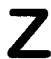
\includegraphics[keepaspectratio]{images/part001_5bbbde23.jpg}}

Note that this is not so in condition (i): a completely secant sequence for A is not necessarily A-regular (exerc. 1).

\begin{enumerate}
\def\labelenumi{\arabic{enumi})}
\setcounter{enumi}{1}
\tightlist
\item
  Let A be a ring, J a finitely generated ideal of A, and p a prime ideal of A containing J. By cor. 2 of th. 1 of § 1, no. 3, we have

\[
\operatorname{prof} _ {A _ {\mathfrak {p}}} (J _ {\mathfrak {p}}; A _ {\mathfrak {p}}) \leqslant [ \kappa (\mathfrak {p}) \otimes_ {A} J: \kappa (\mathfrak {p}) ],
\]

and there is equality if and only if J is completely secant at p.
\end{enumerate}

Suppose that J is distinct from A and generated by a completely secant sequence \((x_{1},\ldots,x_{r})\) . Then we have (prop. 4 of § 1, no. 3, and prop. 1 above)

\[
\operatorname{prof} _ {A} (J; A) = \inf _ {\mathfrak {p} \in V (J)} \operatorname{prof} _ {A _ {\mathfrak {p}}} (J _ {\mathfrak {p}}; A _ {\mathfrak {p}}) = r.
\]

If moreover A is Noetherian, we have \(\operatorname{codim}(\mathrm{V}(\mathrm{J}),\operatorname{Spec}(\mathrm{A}))\leqslant r\) (VIII, § 3, no. 3, prop. 4) and \(\operatorname{prof}_{\mathrm{A}}(\mathrm{J};\mathrm{A})\leqslant \operatorname{codim}(\mathrm{V}(\mathrm{J}),\operatorname{Spec}(\Lambda))\) (§ 1, no. 7, prop. 12), whence finally

\[
\operatorname{prof} _ {\mathrm{A}} (\mathrm{J}; \mathrm{A}) = r = \operatorname{codim} (\mathrm{V} (\mathrm{J}), \operatorname{Spec} (\mathrm{A})) = \operatorname{ht} (\mathrm{J}).
\]

